\documentclass{article}
\usepackage{amsmath}
\usepackage{amsfonts}
\usepackage{amssymb}
\usepackage{multicol}
\usepackage{graphicx}

\graphicspath{ {./images/} }

\setlength{\parindent}{0pt}

\begin{document}

\section*{04/01/2024}
\subsection*{PHYS31.01: Analytical Physics I}
        \begin{enumerate}
            \item \textbf{Rolling w/o Slipping}
            \begin{center}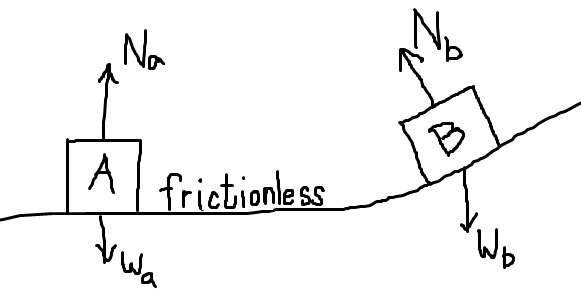
\includegraphics[width=10cm, height=5cm]{1.PNG}\end{center}
            - Given $\omega$ angular velocity, and points $O$ and $P$ on the radius $R$ of a rolling object with angle $\theta$, the distance traveled by the object is equal to:
            \begin{align*}
                d&=r\theta
            \end{align*}
            - That is, assuming the following conditions:
            \begin{align*}
                v_{CM}&=r\omega \\
                a_{CM}&=r\alpha
            \end{align*}
            -There must be a frictional force that holds the contact point in place, and we call it "rolling friction."
            \begin{align*}
                f_r&=\mu_rN
            \end{align*}
            -If the object has rotational and translational motion is in the case of rolling without slipping, the kinetic energy of the rolling object must be written as:
            \begin{align*}
                K=\frac{1}{2}I{\omega}^2+\frac{1}{2}M{v_{CM}}^2
            \end{align*}
            \item \textbf{Example 1: Rolling on inclined plane}
            \begin{center}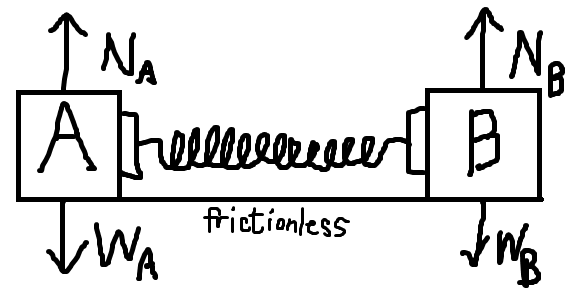
\includegraphics[width=10cm, height=5cm]{2.PNG}\end{center}
            The circular object is rolling without slipping on the ramp. What is the linear speed of the object when it reaches the bottom of the ramp?
            \begin{enumerate}
                \item Method 1. Using torque.
                \begin{center}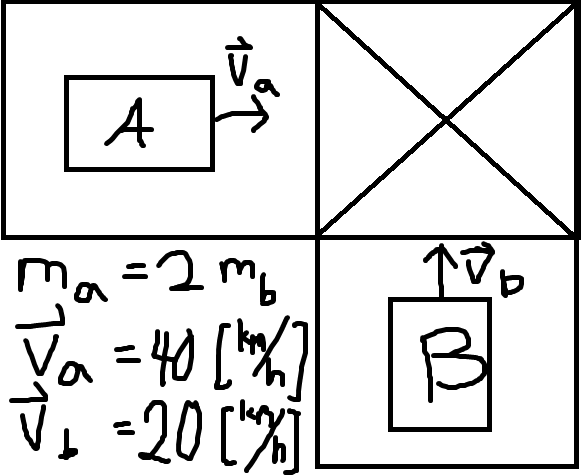
\includegraphics[width=10cm, height=5cm]{3.PNG}\end{center}
                \begin{align*}
                    \textit{Torque is defined as:} \\
                    \vec{\tau}&=\vec{r}\times\vec{F} \\
                    |\vec{\tau}|&=|\vec{r}||\vec{F}|sin\theta \\
                    \textit{Eqns of motion:} \\
                    \textit{Along x: } mgsin\theta-f_r&=ma_{CM} \\
                    \textit{Rotational Motion: } |\tau_{fr}|&=-|r||f_r|sin90\deg \\
                    &=-rf_r \\\\
                    \vec{\tau}_{net}&=I\vec{\alpha} \\
                    -rf_r&=-\gamma mr\alpha &(\textit{where } I=\gamma mr^2)\\
                    f_r&=\gamma ma_{CM} \\\\
                    \textit{Eqn 1 becomes:} \\
                    mgsin\theta-\gamma ma_{CM}&=ma_{CM} \\
                    a_{CM}&=\frac{gsin\theta}{1+\gamma} \\
                    L&=hcsc\theta \\
                    {v_f}^2&={v_i}^2+2a\Delta x \\
                    v_{CM}&=\sqrt{2(\frac{gsin\theta}{1+\gamma})hcsc\theta} \\
                    v_{CM}&=\sqrt{\frac{2gh}{1+\gamma}}
                \end{align*}
                \item Method 2. Conservation of energy:.
                \begin{align*}
                    E_i&=U_i+K_i=mgh&\textit{(topmost portion of the ramp)} \\
                    E_f&=U_f+K_f=\frac{1}{2}{mv_{CM}}^2+\frac{1}{2}I\omega^2&\textit{(bottom of the ramp)} \\
                    E_i&=E_f \\
                    mgh&=\frac{1}{2}{mv_{CM}}^2+\frac{1}{2}I\omega^2 \\
                    &=\frac{1}{2}{mv_{CM}}^2+\frac{1}{2}\gamma mr^2\omega^2 \\
                    gh&=\frac{1}{2}({v_{CM}}^2+\gamma{v_{CM}}^2) &(v_{CM}=r\omega) \\
                    v_{CM}&=\sqrt{\frac{2gh}{1+\gamma}}
                \end{align*}
                \item \textbf{Example 2: Yoyo}
                \begin{center}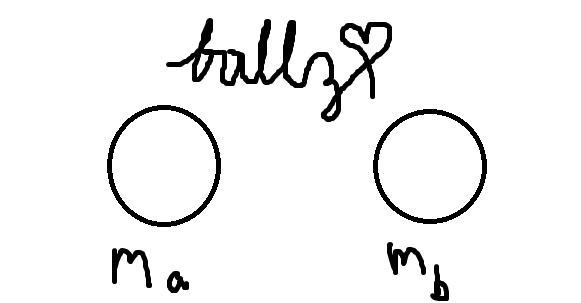
\includegraphics[width=10cm, height=5cm]{4.PNG}\end{center}
                    %%@photo
            \end{enumerate}
            \item \textbf{Angular Momentum}
            - angular momentum is defined as:
            \begin{align*}
                \vec{L}&=\vec{r}\times\vec{p}
                \textit{With $\vec{L}$ pointing into the page.}
            \end{align*}
            If the object is rotating about its COM, then:
            \begin{align*}
                \vec{L}&=I\vec{\omega}
            \end{align*}
            Direction of rotation:
            \begin{align*}
                \vec{\omega}&=-\omega\hat{k}
            \end{align*}
        \end{enumerate}
\end{document}